\section{\texorpdfstring{Tổng quan các công trình nghiên cứu liên quan}{Content}}
Việc tạo sinh dữ liệu mới trong thời gian gần đây đã phát triển mạnh mẽ với sự ra đời của kiến trúc mạng GANs. Hệ thống mạng GANs bao gồm các mạng học máy, học sâu nhỏ hơn, chia thành hai thành phân là mạng tạo sinh dữ liệu (mạng G) và mạng phân biệt dữ liệu (mạng D). Mạng G đóng vai trò như khối Decoder trong bộ Variational Autoencoder \cite{vae_base},  có chức năng học và xấp xỉ được phân phối xác suất của dữ liệu gốc, từ đó tạo sinh ra dữ liệu mới giữ được đặc trưng và tương đồng với dữ liệu gốc. Mạng D có chức năng phân biệt giữa dữ liệu được tạo sinh bởi mạng G và tập dữ liệu huấn luyện. Trong quá trình huấn luyện, dựa trên hàm mất mát của D, các trọng số của cả hai mạng G và D đều được cập nhật trong quá trình lan truyền ngược, từ đó giúp hai mạng này tăng độ chính xác. Với mạng G, qua quá trình huấn luyện, mạng sẽ có khả năng tạo sinh ra được dữ liệu ngày càng chân thực hơn, khó phân biệt hơn. Trong khi đó, mạng D cũng ngày càng có chức năng phân biệt tốt hơn, chuẩn xác hơn. Đến một lúc nào đó, độ chính xác của hai mạng sẽ đạt đến mức cân bằng, lúc này hai mạng đã hội tụ và không thể được cải thiện hơn với kiến trúc mạng và tập dữ liệu huấn luyện hiện tại, nên ta sẽ dừng quá trình huấn luyện tại đây.

%------------------------------------------------------------------------

\subsection{\texorpdfstring{Bài nghiên cứu "Lip Movements Generation at a Glance"\cite{chen2018}}{Target}}

\begin{figure}[H]
    \centering
    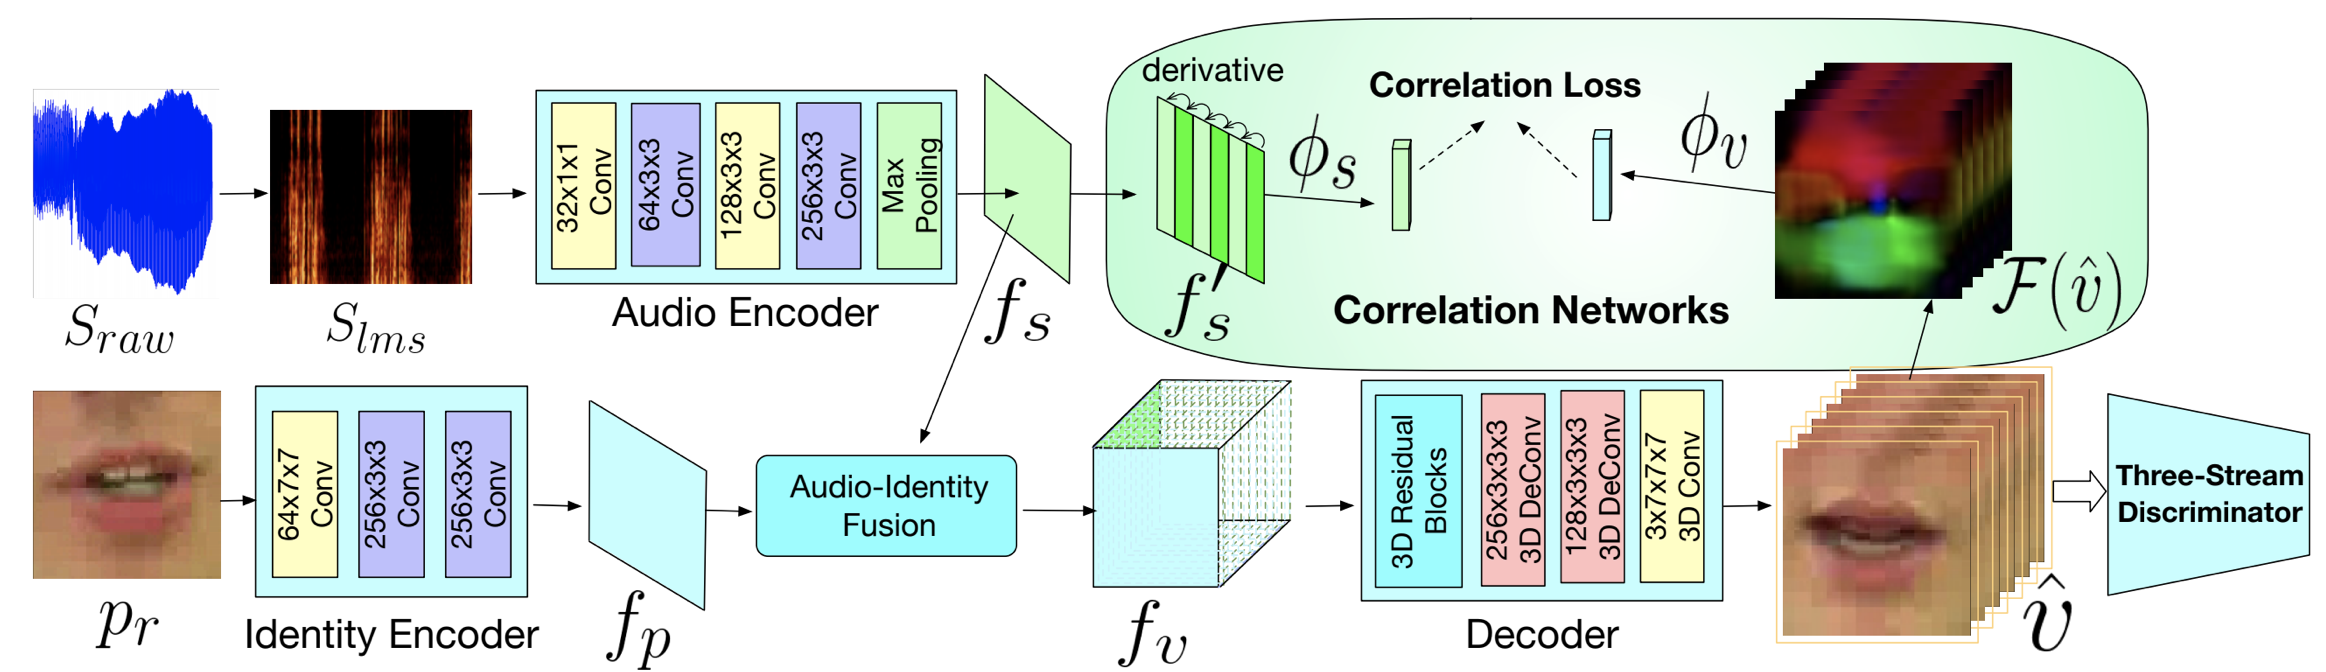
\includegraphics[width=15cm]{./content/images/chen2018_model.png}
    \caption{Mô hình của bài báo Lip Movements Generation at a Glance}
    \label{fig:chen2018_model}
\end{figure}

Việc tạo sinh khẩu hình miệng khớp với tiếng nói là bước đầu tiên để thực hiện việc tạo sinh khuôn mặt. Nghiên cứu này đã thành công trong việc tạo sinh khẩu hình miệng từ một ảnh tĩnh chứa hình ảnh khuôn miệng của một người bất kỳ, và một đoạn âm thanh chứa tiếng nói. Bằng phương pháp kết hợp các đặc trưng âm thanh và hình ảnh, nghiên cứu cho ra kết quả tốt và có độ chính xác cao hơn so với các nghiên cứu trước đó. Hình \ref{fig:chen2018_model} mô tả cấu trúc của mạng tạo sinh ảnh được dùng. Đầu tiên, âm thanh được cắt thành các đoạn nhỏ dài 0.64s, các đoạn này được chuyển thành phổ Log-Mel ($S_{raw}$ thành $S_{lms}$), sau đó qua một bộ Audio Encoder để trích đặc trưng, ta có đặc trưng âm thanh $f_s$ là một ma trận 2 chiều kích thước $F \times T$. Bên cạnh đó, hình ảnh khuôn miệng cũng được đưa qua một bộ Identity Encoder để tạo thành ma trận 2 chiều $f_p$ kich thước $H \times W$.

\begin{figure}[H]
    \centering
    \begin{minipage}{0.48\textwidth}
        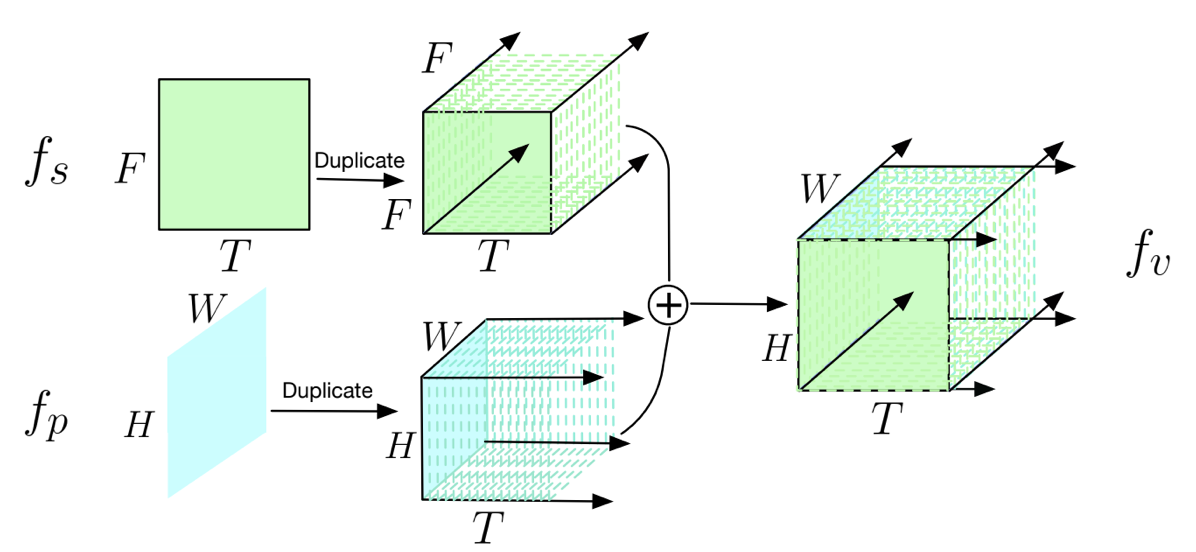
\includegraphics[width=7cm]{./content/images/chen2018_fusion.png}
        \caption{Phương pháp kết hợp đặc trưng hình ảnh và âm thanh}
        \label{fig:chen2018_fusion}
    \end{minipage}\hfill
    \begin{minipage}{0.48\textwidth}
        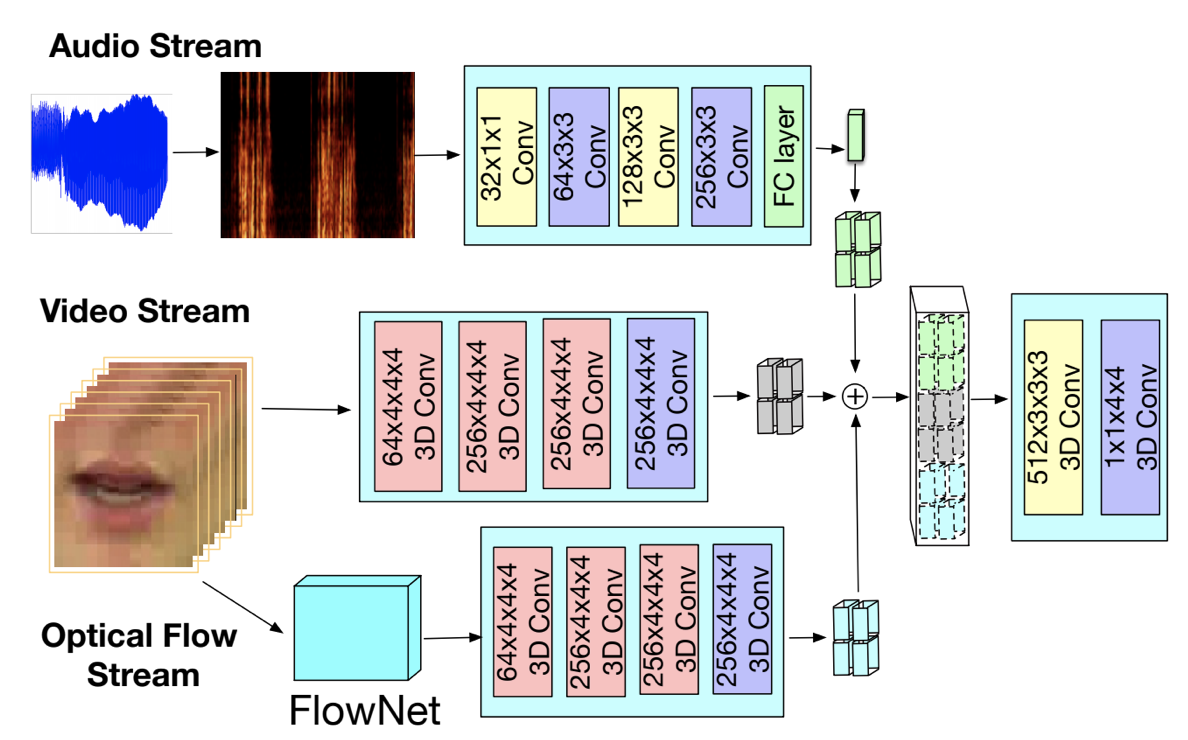
\includegraphics[width=7cm]{./content/images/chen2018_gans.png}
        \caption{GANs Discriminator với 3 loại đặc trưng}
        \label{fig:chen2018_gans}
    \end{minipage}
\end{figure}

Để kết hợp hai đặc trưng hình ảnh, âm thanh với nhau để tạo sinh hình ảnh mới, tác giả bài báo đề xuất phương pháp nhân bản ma trận $f_s$ F lần và nhân bản ma trận $f_p$ T lần thành hai tensor ba chiều, sau đó nối tiếp các kênh của hai tensor này để tạo thành khối tensor ba chiều mới. Để có thể nối tiếp được với nhau, Tác giả đã đặt các thông số $H = W = F$. Hình \ref{fig:chen2018_fusion} miêu tả cách kết hợp hai đặc trưng hình ảnh - âm thanh thành khối đặc trưng chung $f_v$, khối $f_v$ có kích thước $W \times H \times T$. Khối đặc trưng này sau cùng được chuyển đổi thành ảnh đầu ra $\hat{v}$ nhờ vào mạng Decoder. Mạng Decoder này sử dụng kiến trúc 3D Residual và các khối Deconvolution nhằm bảo toàn các đặc điểm của hình ảnh gốc.

Đồng thời, nghiên cứu này cũng chỉ ra rằng đặc tính của khuôn miệng trong video là hình ảnh thường đi trước âm thanh, và độ trễ âm thanh - hình ảnh là không đồng nhất trong các video khác nhau. Vì vậy, để tạo sinh một video chân thực, ta phải quan tâm đến độ trễ này. Khối Correlation Network trong hình \ref{fig:chen2018_model} miêu tả cách tính toán giá trị Corellation Loss. Để tính giá trị này, bộ tính toán cần có một encoder ($\phi_s$) để encode sự thay đổi của âm thanh và một encoder ($\phi_v$) để encode sự thay đổi của hình ảnh. Ma trận $f_s$ được tính đạo hàm theo trục T thành $f'_s$, hình ảnh được tạo sinh $\hat{v}$ cũng được đưa qua hàm $\mathcal{F}$ để lấy đặc trưng Optical Flow. Sau đó, cả hai đặc trưng thể hiện sự thay đổi của âm thanh và hình ảnh theo thời gian này được đưa qua các encoder $\phi_s$ và $\phi_v$ để tạo ra hai vector có cùng số chiều.Công thức tính của giá trị Correlation Loss chính là hiệu của 1 và giá trị cosin giữa hai vector đặc trưng cuối cùng:

\begin{equation}
    \ell_{corr} = 1 - \frac{\phi_s(f'_s)\cdot\phi_v(\mathcal{F}(v))}{\|\phi_s(f'_s)\|_2\cdot\|\phi_v(\mathcal{F}(v))\|_2}
    \label{eqn:chen2018_corr_loss}
\end{equation}


Cấu trúc mạng GANs cũng đã được sử dụng trong nghiên cứu này nhằm mục đích tạo ra chuyển động mượt mà cho chuỗi hình ảnh trong video và làm cho chất lượng ảnh tạo sinh tốt hơn. Bộ phân biệt (Discriminator) giữa ảnh thật và ảnh tạo sinh ($D$) được miêu tả trong hình \ref{fig:chen2018_gans}. Đặc trưng Log-Mel của âm thanh được encode thành một vector bằng một mạng Convolution - Fully connected, sau đó vector này được nhân bản và ghép nối để có số chiều bằng với tensor của hai đặc trưng còn lại. Hình ảnh được đưa vào mạng được encode bởi các khối 3D Convolution để có được tensor đặc trưng ảnh. Các ảnh này cũng được đưa qua mạng FlowNet để đưa ra đặc trưng Optical Flow, đặc trưng này cũng được encode để tạo ra tensor đặc trưng cho chuyển động trong video. Sau cùng, ba đặc trưng này được ghép nối tiếp theo kênh và được đưa qua các khối 3D Convolution để lấy được xác suất dự đoán ảnh thật hay tạo sinh của mạng. Cặp video - âm thanh đưa vào mạng có thể là video thật và đoạn âm thanh khớp với video đó, hoặc video thật và một đoạn âm thanh khác, hoặc video được tạo sinh và đoạn âm thanh tương ứng tạo ra nó. Hàm mất mát của mạng được định nghĩa như sau:

\begin{equation}
    \ell_{dis} = -logD([s^j, v^j]) - \lambda_plog(1 - D([s^j, \hat{v}])) - \lambda_ulog(1 - D([s^j, v^k])), k \ne j
\end{equation}

Để so sánh sự tương đồng về mặt tổng quan giữa hai video (video thật và video được tạo sinh), tác giả sử dụng một bộ Autoencoder. Bộ Autoencoder này được huấn luyện độc lập với mạng chính và sử dụng cùng bộ dữ liệu với mạng chính. Phần encoder ($\varphi$) được giữ lại để encode hình ảnh từ video nhằm mục đích trích xuất đặc trưng của chuỗi hình ảnh. Hàm Perceptual Loss $\ell_{perc}(\hat{v}, v)$ được dùng để tính toán độ sai lệch về mặt tổng quan giữa video được tạo sinh từ tiếng nói và video thật tương ứng với tiếng nói:
\begin{equation}
    \ell_{perc}(\hat{v}, v) = \|\varphi(v) - \varphi(\hat{v})\|^2_2
    \label{eqn:chen2018_perc_loss}
\end{equation}

Hàm mất mát của cuối cùng của mạng được định nghĩa:
\begin{equation}
    \mathcal{L} = \ell_{corr} + \lambda_1\ell_{pix} + \lambda_2\ell_{perc} + \lambda_3\ell_{gen}
    \label{eqn:chen2018_loss}
\end{equation}

Trong đó:
\begin{itemize}
\item $\ell_{corr}$: Là giá trị mất mát do sự sai lệch giữa hình ảnh và âm thanh đã nêu ở (\ref{eqn:chen2018_corr_loss}).
\item $\ell_{pix}$: Giá trị mất mát dựa trên sự sai khác ở cấp độ điểm ảnh giữa ảnh được tạo sinh và ảnh trong video thật, $\ell_{pix} = \|v-\hat{v}\|$.
\item $\ell_{perc}$: Giá trị mất mát đo độ sai khác trên toàn bộ chuỗi hình ảnh (đã nêu ở (\ref{eqn:chen2018_perc_loss})).
\item $\ell_{gen}$: Giá trị mất mát của bộ tạo sinh ảnh dựa trên hàm phân biệt $D$: $\ell_{gen} = -logD([s^j, \hat{v}^j])$.
\end{itemize}

Mô hình được huấn luyện và kiểm thử trên các tập dữ liệu GRID, LDC và LRW. Kết quả kiểm thử cho thấy mô hình này cho kết quả tạo sinh hình ảnh tốt hơn hẳn so với các nghiên cứu trước đó. Các độ đo PSNR, SSIM, LMD và CPBD (đã nêu ở phần \ref{sec:metrics_eval}) được sử dụng để kiểm chứng. Sau đây là kết quả được khảo sát bới tác giả:

\begin{figure}[H]
    \centering
    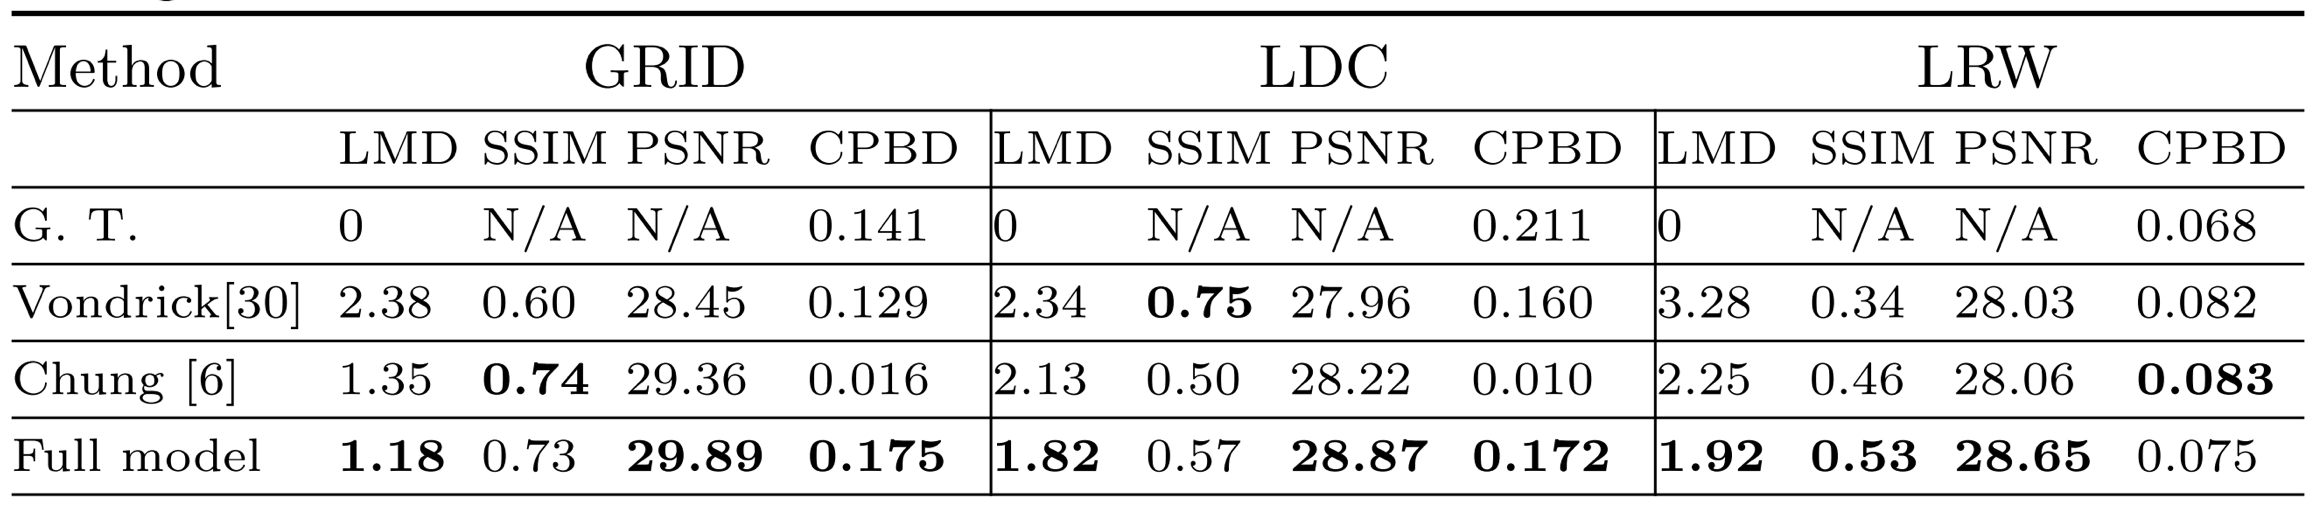
\includegraphics[width=15cm]{./content/images/chen2018_result.png}
    \caption{Kết quả đánh giá và so sánh mô hình trong nghiên cứu Lip Movements Generation at a Glance}
    \label{fig:chen2018_result}
\end{figure}

Nghiên cứu này đã đưa ra các phương pháp phù hợp và tiến bộ để trích xuất và kết hợp đặc trưng hình ảnh và âm thanh, đồng thời cũng tận dụng phương pháp GANs để cải thiện chất lượng của ảnh được tạo sinh. Độ hiệu quả của cấu trúc mạng được thể hiện qua kết quả đo lường vượt trội so với các nghiên cứu cùng thời điểm. Tuy nhiên, cấu trúc mạng này có một số yếu điểm. Thứ nhất, mạng chỉ có thể nhận vào hình ảnh tĩnh và một đoạn âm thanh có độ dài xác định (0.64s) và cho ra số khung hình tương ứng với khoảng thời gian đó (16 khung hình). Thứ hai, tác giả vẫn chưa chú ý đến hiện tượng jittering của video được tạo sinh, mạng không có cơ chế để đảm bảo việc chuyển ảnh mượt mà, ít sai khác về độ tương phản, ánh sáng, màu sắc giữa các khung ảnh gần nhau.

%------------------------------------------------------------------------

\subsection{\texorpdfstring{Bài nghiên cứu "End-to-End Speech-Driven Facial Animation with Temporal GANs"\cite{vougioukas2019}}{Target}}
\label{sec:vougioukas2019}

\begin{figure}[H]
    \centering
    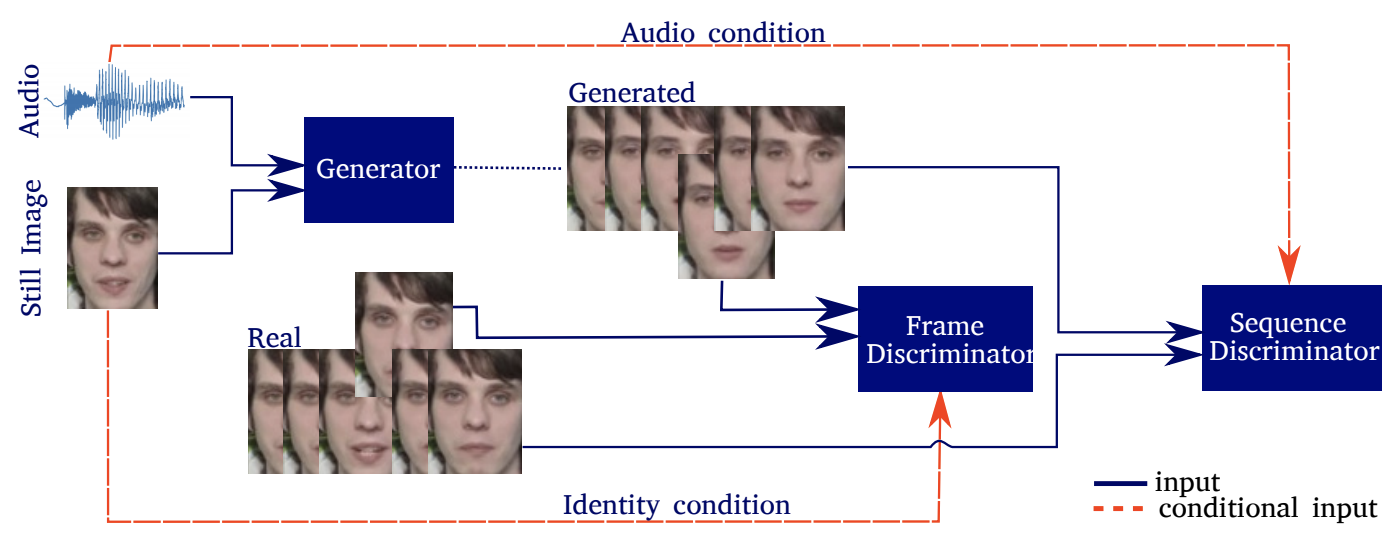
\includegraphics[width=15cm]{./content/images/vou2019_model.png}
    \caption{Mô hình của nghiên cứu End-to-End Speech-Driven Facial Animation with Temporal GANs}
    \label{fig:vou2019_model}
\end{figure}

Nghiên cứu của Vougioukas vào năm 2019 có mục tiêu là tạo ra chuỗi hình ảnh của toàn bộ gương mặt người đang nói với đầu vào là một ảnh tĩnh chứa mặt người bất kỳ và một đoạn tiếng nói bất kỳ. Kiến trúc của mạng được miêu tả trong hình \ref{fig:vou2019_model}, được bao gồm ba phần chính. Bộ tạo sinh ảnh Generator nhận vào một đoạn âm thanh tiếng nói có độ dài bất kỳ và một ảnh tĩnh, sử dụng những dữ liệu này như một gợi ý để tạo sinh chuỗi hình ảnh mới với mặt người đang nói tiếng nói tương ứng. Bộ phân biệt ảnh theo khung hình Frame Discriminator cũng nhận vào ảnh tĩnh nói trên, đồng thời nhận thêm một ảnh khác, ảnh này hoặc được tạo sinh từ Generator, hoặc được trích xuất từ video trong bộ dữ liệu. Frame Discriminator sẽ được huấn luyện để phân biệt đâu là ảnh được tạo sinh và đâu là ảnh thật được trích xuất từ video huấn luyện. Bộ phân biệt chuỗi ảnh Sequence Discriminator nhận vào đoạn tiếng nói và một chuỗi hình ảnh trong video. Chuỗi hình ảnh này có thể là hình ảnh được tạo sinh hoặc hình ảnh gốc từ video tương ứng. Bộ Sequence Discriminator sẽ học cách phân biệt hai loại video này trong quá trình huấn luyện. Theo như cơ chế GANs, trong quá trình huấn luyện, hàm mất mát của hai bộ Discriminator sẽ tạo ra lan truyền ngược và cập nhật trọng số của chính nó và của cả Generator. Từ đó, cả ba mạng này đều sẽ dần trở nên chính xác hơn.

\begin{figure}[H]
    \centering
    \begin{minipage}{0.48\textwidth}
        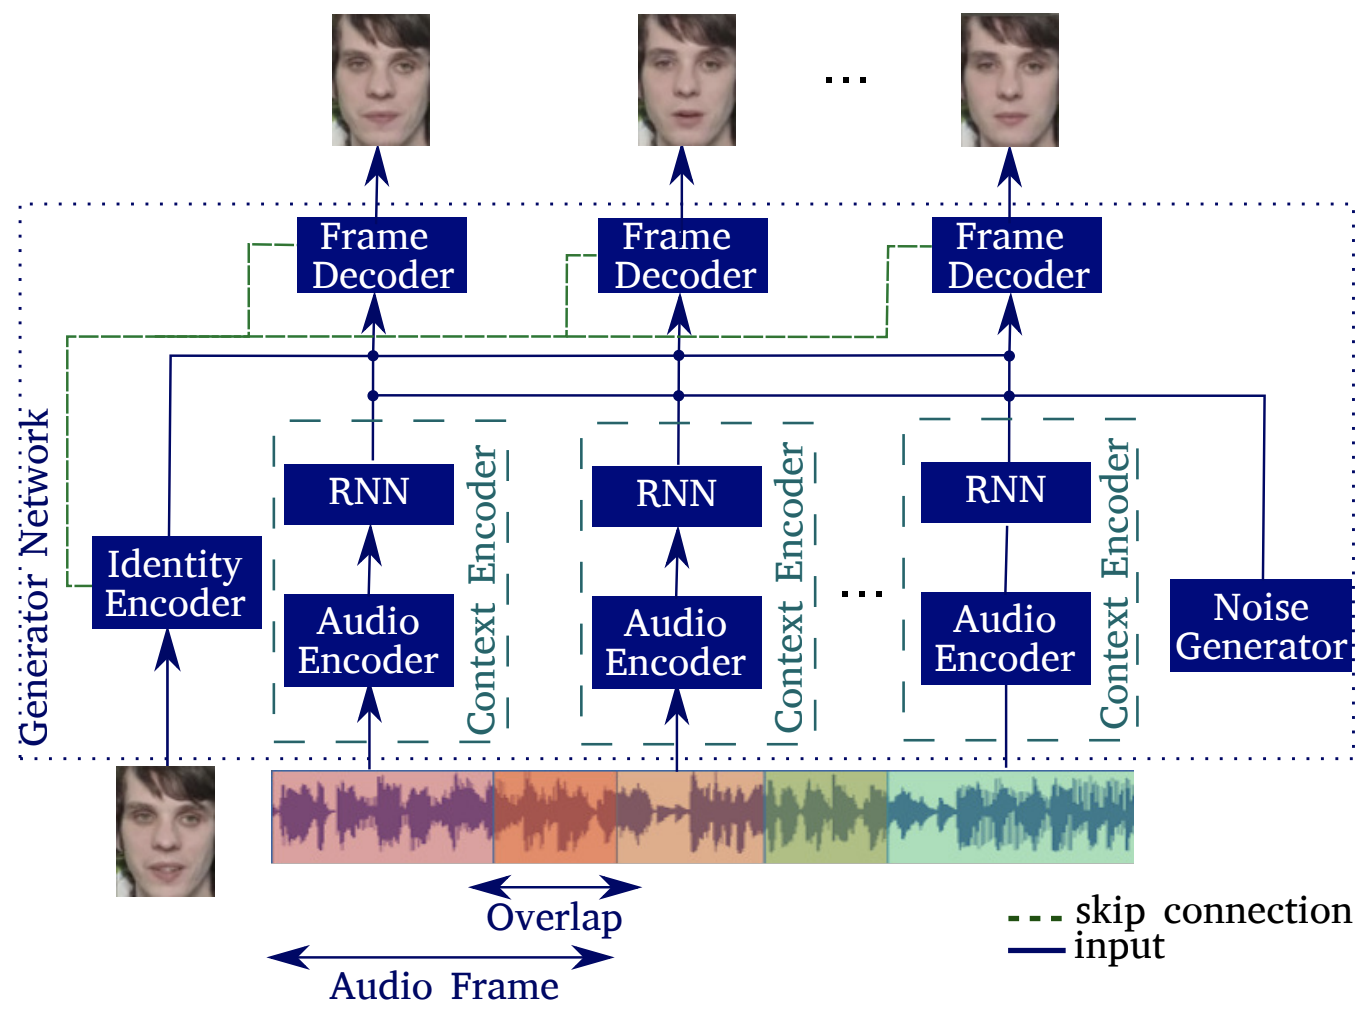
\includegraphics[width=7cm]{./content/images/vou2019_gen.png}
        \caption{Kiến trúc bộ Generator}
        \label{fig:vou2019_gen}
    \end{minipage}\hfill
    \begin{minipage}{0.48\textwidth}
        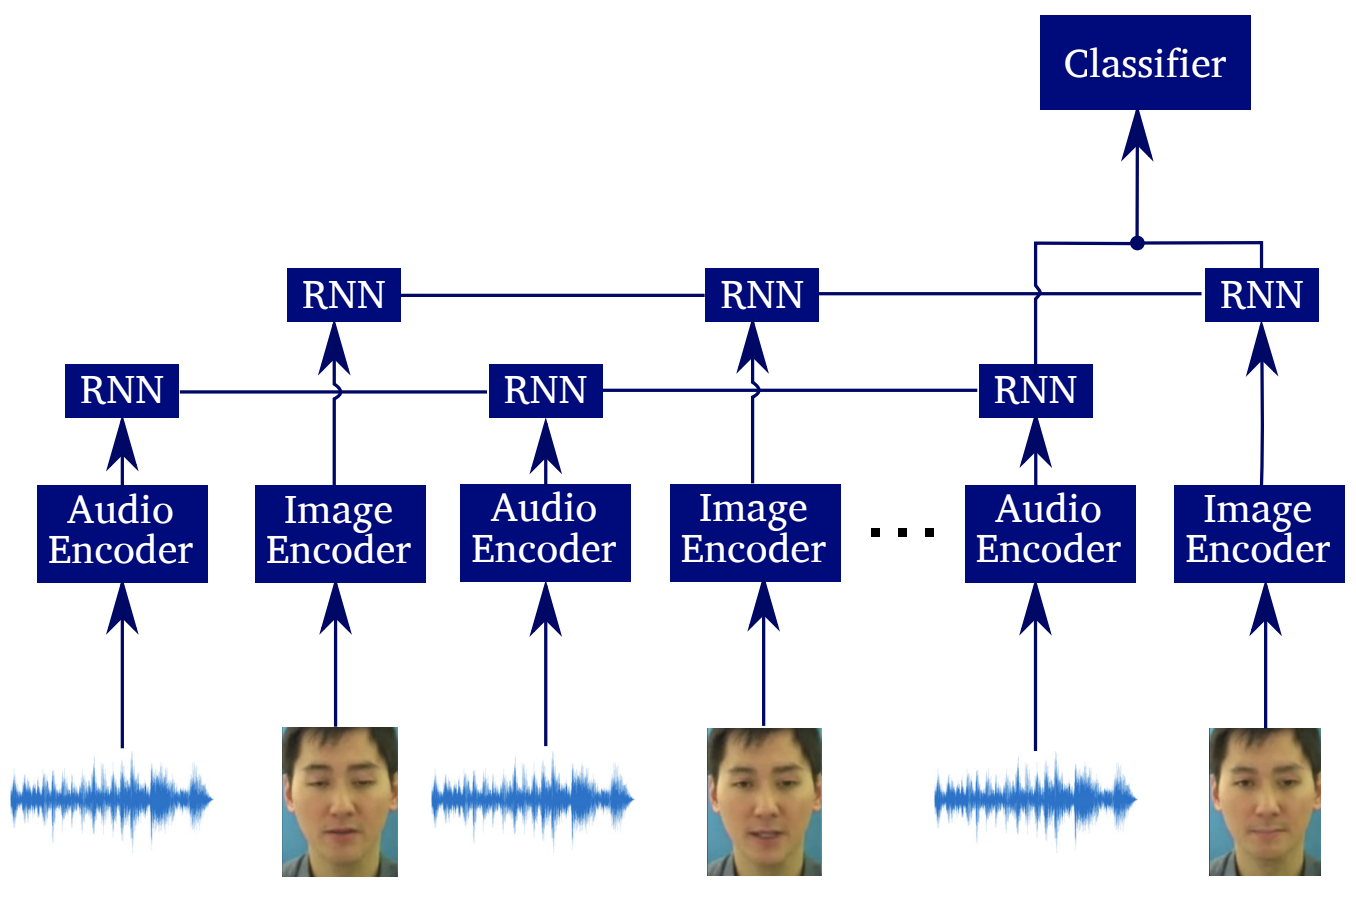
\includegraphics[width=7cm]{./content/images/vou2019_seq_dis.png}
        \caption{Kiến trúc bộ Sequence Discriminator}
        \label{fig:vou2019_seq_dis}
    \end{minipage}
\end{figure}

Trong nghiên cứu này, video huấn luyện được tách riêng thành âm thanh và hình ảnh. Mỗi khung hình kích thước $96\times128$ được cắt ra từ video tương ứng với đoạn âm thanh dài 0.16s, đoạn âm thanh này tạo thành một vector 8000 điểm. Như vậy, dữ liệu được tiền xử lý bằng cách cắt nhỏ video thành khung ảnh và đoạn âm thanh tương ứng với ảnh đó (âm thanh có chồng lấn giữa các ảnh).

Kiến trúc của bộ tạo sinh chuỗi ảnh Generator được miêu tả trong hình \ref{fig:vou2019_gen}. Identity Encoder là bộ encoder ảnh có tính năng trích xuất đặc trưng của ảnh tĩnh được đưa vào mạng. Bộ encoder này gồm 6 lớp 2D Convolution, mỗi lớp kết hợp với Batchnorm và ReLU ở phía sau. Mạng này giúp trích xuất ảnh đầu vào thành vector 50 chiều ($z_{id}$). Context Encoder là tổng hợp của hai bộ bao gồm Audio Encoder và một bộ RNN hai lớp. Audio Encoder sẽ trích xuất đặc trưng từ đoạn âm thanh 8000 điểm (vector 8000 chiều) để tạo ra vector 256 chiều. Đặc trưng này được đưa vào bộ RNN để bổ sung ngữ nghĩa về mặt thời gian. Ngõ ra của bộ Context Encoder là trạng thái ẩn (hidden state) của bộ RNN có số chiều bằng 256 ($z_c$). Generator còn có một bộ Noise Generator, thực chất là một mạng GRU có chức năng tạo ra vector nhiễu Gauss 10 chiều ($z_n$). $z_{id}$, ($z_c$) và ($z_n$) được ráp nối với nhau theo kênh tương ứng trước khi đưa vào bộ tạo sinh ảnh. Trong khi $z_{id}$ có chức năng giúp Frame Decoder tái tạo chính xác gương mặt của người nói, $z_c$ sẽ mang thông tin về mặt âm thanh, thời gian và hoàn cảnh, giúp tạo ra gợi ý cho mạng để tạo sinh được hình ảnh tương ứng với âm thanh. Đồng thời, $z_n$ tạo ra tính ngẫu nhiên cho mạng, khi đưa cùng một đầu vào, thì sẽ không khi nào mạng cho ra kết quả giống nhau ở hai lần thử. Đồng thời, tính ngẫu nhiên này lại có tính chất phụ thuộc thời gian (do được tạo ra bởi mạng GRU) đem lại cho hình ảnh được tạo sinh các biểu cảm nhỏ như nháy mắt và các chuyển động nhỏ trên mặt một cách liền lạc.

Ở đầu ra, bộ sinh ảnh Frame Decoder được sử dụng để tạo sinh chuỗi ảnh theo thời gian. Vector đặc trưng ẩn có 316 chiều, từ vector đặc trưng này, Frame Decoder sẽ tạo ra hình ảnh có kích thước bằng với hình mẫu ban đầu ($96\times128$). Nhằm bảo toàn nhận dạng của người trong ảnh mẫu, Frame Decoder được thiết kế theo kiến trúc U-Net gồm 6 lớp Convolution tương ứng với Identity Encoder. Các lớp Convolution này nhận thêm các đặc trưng ẩn từ lớp tương ứng của Identity Encoder để hạn chế việc đánh mất nhận dạng của mặt người mẫu do bị ảnh hưởng bởi độ sâu cũa mạng. Các đặc trưng ẩn đi qua các lớp Deconvolution và cuối cùng tạo ra ảnh tương ứng với âm thanh.

Bộ phân biệt khung ảnh Frame Discriminator trong hình \ref{fig:vou2019_model} là một mạng Convolution 6 lớp, đầu ra của mạng là xác suất ảnh này được cho là ảnh được tạo sinh. Frame Discriminator giúp cho ảnh tạo sinh từ Generator chân thực hơn, khó phân biệt với ảnh từ video gốc hơn. Bộ phân biệt chuỗi ảnh Sequence Discriminator được miêu tả trong hình \ref{fig:vou2019_seq_dis} có cấu trúc trích xuất đặc trưng tương tự như bộ Generator. Sự khác biệt đến từ bộ trích xuất đặc trưng chuỗi ảnh. Chuỗi hình ảnh được đưa qua bộ Image Encoder để trích xuất đặc trưng ảnh và thu nhỏ số chiều dữ liệu. Các ảnh sau khi qua bộ Image Encoder sẽ được đưa vào mạng RNN hai lớp để cập nhật trạng thái ẩn của mạng RNN. Khi kết thúc chuỗi hình ảnh và âm thanh tương ứng với nó, trạng thái ẩn của hai mạng RNN cho âm thanh và RNN cho hình ảnh được ghép nối tiếp vào nhau theo kênh. Lúc này, đặc trưng âm thanh giúp làm điều kiện để phân biệt chuỗi ảnh tốt hơn. Một bộ Classifier được sử dụng để tính toán xác suất chuỗi ảnh được đưa vào có phải chuỗi được tạo sinh hay không. Bộ Sequence Discriminator giúp cho video tạo ra có sự chân thật trong các chuyển động của khuôn mặt, cũng như sự chân thật trong sự chuyển tiếp giữa các khung hình, nhờ đó tránh được hiện tượng nhảy hình bất thường.

Trong quá trình huấn luyện, các ảnh từ video được cho vào Frame Discriminator ($D_{img}$) bằng cách lấy mẫu với xác suất đều qua hàm $S(x)$ trên chuỗi ảnh $x$. Sequence Discriminator ($D_{seq}$) sẽ phân biệt cả chuỗi ảnh $x$ và âm thanh $a$. Hàm mất mát của GANs được biểu diễn như sau:

\begin{equation}
    \begin{split}
    \mathcal{L}_{adv}(D_{img},D_{seq},G) = &\mathrm{E}_{x\sim P_d}[logD_{img}(S(x),x_1)] + \mathrm{E}_{z\sim P_z}[log(1 - D_{img}(S(G(z)), x_1))] + \\
    &\mathrm{E}_{x\sim P_d}[logD_{seq}(x,a)] + \mathrm{E}_{z\sim P_z}[log(1 - D_{seq}(G(z), a))]
    \end{split}
    \label{eqn:vou2019_adv_loss}
\end{equation}

Hàm mất mát L1 cũng được dùng trên một nửa dưới của ảnh để đảm bảo ảnh được tạo sinh có hình ảnh thể hiện chân thật khuôn miệng và khẩu hình miệng phù hợp với lời nói. Hàm mất mát L1 được biểu diễn như sau:

\begin{equation}
    \mathcal{L}_{L1} = \sum_{p\in[0,W]\times[\frac{H}{2},H]}\vert F_p - G_p \vert
    \label{eqn:vou2019_l1_loss}
\end{equation}

Như vậy, mục tiêu của cả hệ thống là giảm thiểu hàm mất mát chung bằng cách điều chỉnh các trọng số của bộ tạo sinh ảnh Generator ($G$) và các bộ phân biệt ảnh Discriminator ($D$). Hàm mục tiêu của mạng được biểu diễn như sau:

\begin{equation}
    \mathrm{arg}\: \underset{G}{\mathrm{min}}\: \underset{D}{\mathrm{max}}\: \mathcal{L}_{adv} + \lambda\mathcal{L}_{L1}
    \label{eqn:vou2019_loss}
\end{equation}

Sau đây là bảng so sánh của tác giả với các thông số PSNR, SSIM, CPBD, WER và một số độ đo khác. Bài nghiên cứu cũng so sánh kết quả của họ với một nghiên cứu trước đó (Baseline):

\begin{figure}[H]
    \centering
    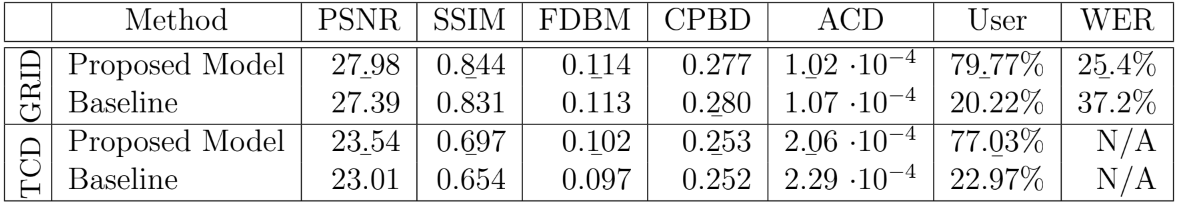
\includegraphics[width=15cm]{./content/images/vou2019_result.png}
    \caption{Kết quả của nghiên cứu End-to-End Speech-Driven Facial Animation with Temporal GANs}
    \label{fig:vou2019_result}
\end{figure}

Mô hình trong bài nghiên cứu đem lại tín hiệu khả quan cho việc tạo sinh ảnh khuôn mặt dựa trên tiếng nói. Phương pháp tạo sinh và các bộ phân biệt ảnh áp dụng phương pháp CGANs một cách hiệu quả nhẳm mục đích tạo sự chân thật cho chuỗi ảnh. Một số kết quả được công bố bởi tác giả bài nghiên cứu cho thấy ảnh được tạo sinh có chất lượng tốt, không bị hiện tượng nhảy hình, độ ổn định khung hình tốt, có thể đánh lừa người xem qua phép thử Turing. Theo đó, có tới 79.77\% chuỗi hình ảnh bị đánh nhãn sai (được tạo sinh hay video thật) trên tập dữ liệu GRID và 77.03\% trên tập dữ liệu TCD. Tuy nhiên, một số hạn chế vẫn chưa được giải quyết. Thứ nhất, ngoài vùng miệng, bộ tạo sinh hình ảnh và các bộ phân biệt vẫn chưa chú trọng đến các phần khác trong khuôn mặt nhất là phần nửa trên. Điều này làm cho hình ảnh được tạo sinh thiếu tự nhiên so với video thực tế. Thứ hai, khuôn mặt vẫn chưa thể hiện được cảm xúc tương ứng với tiếng nói. Việc này cũng góp phần làm cho video được tạo sinh dễ bị nhận biết bởi người xem tinh ý. Thứ ba, chuyển động của đầu cũng không được thể hiện trong video làm cho video trở nên cứng nhắc và giả tạo nếu chiếu trong thời gian dài. Thứ tư, sự đồng bộ của tiếng nói và hình ảnh chưa được quan tâm và chưa có cơ chế đảm bảo hình ảnh được tạo sinh sẽ được căn giờ chuẩn xác với âm thanh.

%------------------------------------------------------------------------

\subsection{\texorpdfstring{Bài nghiên cứu "Realistic Speech-Driven Facial Animation with GANs"\cite{vougioukas2020}}{Target}}

Đây là bài nghiên cứu có cùng tác giả với bài nghiên cứu trong phần \ref{sec:vougioukas2019}. Với cùng mục tiêu và phương pháp tiếp cận tương đồng với nghiên cứu được công bố  năm 2019, Vougioukas đã có một số cập nhật, bổ sung và đánh giá cho mô hình được xây dựng. Trong nghiên cứu này, Vougioukas đã thêm vào mạng trước đó một bộ phân biệt mới, bộ phân biệt này giúp đảm bảo sự đồng bộ giữa hình ảnh được tạo sinh và tiếng nói tương ứng. Kiến trúc được cập nhật mới thể hiện ở hình \ref{fig:vou2020_model}.

\begin{figure}[H]
    \centering
    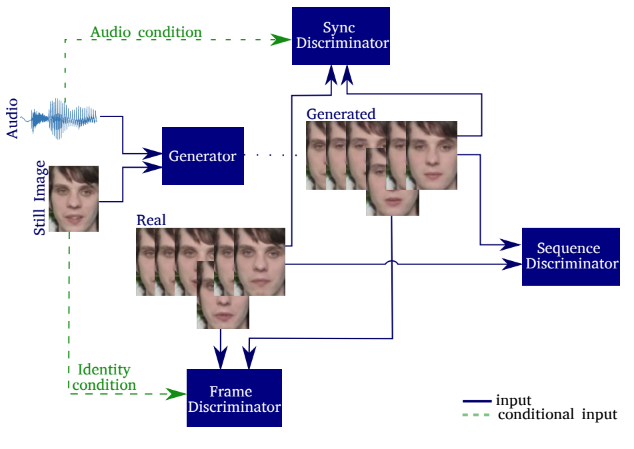
\includegraphics[width=9cm]{./content/images/vou2020_model.png}
    \caption{Kiến trúc mạng được cập nhật trong nghiên cứu mới của Vougioukas}
    \label{fig:vou2020_model}
\end{figure}

Bộ phân biệt tính đồng bộ Sync Discriminator được thể hiện trong hình \ref{fig:vou2020_sync_dis}. Bộ phân biệt này nhận vào một chuỗi hình ảnh nửa dưới (phần ảnh chứa vùng miệng) của mặt người đang nói. Chuỗi hình ảnh này có thể được tạo sinh bởi mạng sinh ảnh Generator hoặc là chuỗi ảnh thật được trích xuất từ video. Đồng thời, mạng cũng nhận vào đoạn tiếng nói tương ứng với chuỗi hình ảnh trên. Dữ liệu đưa vào mạng được thể hiện trong hình \ref{fig:vou2020_sync_input}. Chuỗi hình ảnh được đưa vào gồm 5 ảnh gồm $96 \times 64$ điểm ảnh tạo thành một tensor ba chiều. Tensor này được biến biến đổi thành ma trận hai chiều nhờ một lớp 3D Convolution. Sau đó, ma trận này tiếp tục được trích xuất đặc trưng nhờ ba lớp 2D Convolution và ở cuối là một lớp tuyến tính. Đặc trừng ảnh sau cùng được trích xuất là một vector 256 chiều. Đối với tiếng nói, quy trình trích xuất đặc trưng cũng được áp dụng trên vector âm thanh 8000 chiều. Bộ trích xuất đặc trưng âm thanh được sử dụng bao gồm 5 lớp 1D Convolution và cuối cùng là một lớp tuyến tính. Đặc trưng âm thanh cũng được trích xuất thành một vector 256 chiều. Khoảng cách Euclide giữa hai vector được tính toán theo công thức $d = \Vert \textrm{e}_{\textrm{sm}} - \textrm{e}_{\textrm{a}} \Vert$, với $\textrm{e}_{\textrm{sm}}$ và $\textrm{e}_{\textrm{a}}$ lần lượt là vector đặc trưng chuỗi hình ảnh và vector đặc trưng tiếng nói. Khoảng cách $d$ sau đó được đưa vào một lớp Perceptron để đưa ra sự đo đạc về độ phù hợp giữa chuỗi hình ảnh vùng miệng và âm thanh được đưa vào dưới dạng xác suất.

\begin{figure}[H]
    \centering
    \begin{minipage}{0.48\textwidth}
        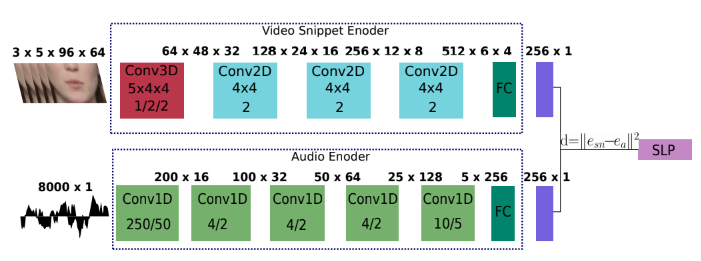
\includegraphics[width=7cm]{./content/images/vou2020_sync_dis.png}
        \caption{Kiến trúc bộ phân biệt đồng bộ Sync Discriminator}
        \label{fig:vou2020_sync_dis}
    \end{minipage}\hfill
    \begin{minipage}{0.48\textwidth}
        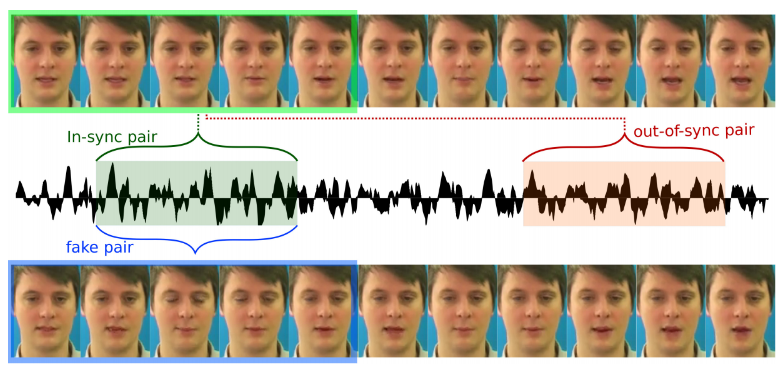
\includegraphics[width=7cm]{./content/images/vou2020_sync_input.png}
        \caption{Miêu tả dữ liệu được đưa vào mạng phân biệt đồng bộ}
        \label{fig:vou2020_sync_input}
    \end{minipage}
\end{figure}

Để có khả năng phân biệt tốt nhất, cặp hình ảnh - tiếng nói được đưa vào mạng được chọn lựa theo ba hoàn cảnh (xem hình \ref{fig:vou2020_sync_input}). Cặp đồng bộ đúng (in-sync pair), là cặp hình ảnh - tiếng nói tương ứng với nhau trong video. Cặp không đồng bộ (out-of-sync pair) gồm hình ảnh được trích xuất từ video nhưng không phù hợp với tiếng nói. Cuối cùng là cặp giả mạo (fake pair) gồm hình ảnh được tạo sinh vào tiếng nói tương ứng tạo sinh ra nó. Nhờ ba cặp này, mạng sẽ học được cách phân biệt sự sai lệch hình ảnh - tiếng nói và đặc biệt là sự đồng bộ của khẩu hình miệng với tiếng nói được cải thiện đáng kể.

Hàm mất mát phân biệt $\mathcal{L}_{adv}$ của mạng cũng được cập nhật thêm hàm mất mát của bộ phân biệt đồng bộ. Qua đó:

\begin{equation}
    \mathcal{L}_{adv} = \lambda_{img}\mathcal{L}^{img}_{adv} + \lambda_{adv}\mathcal{L}^{seq}_{adv} + \lambda_{seq}\mathcal{L}^{seq}_{adv}
    \label{eqn:vou2020_adv_loss}
\end{equation}

Với:

\begin{equation}
    \mathcal{L}^{img}_{adv} = \mathrm{E}_{x\sim P_d}[logD_{img}(S(x),x_1)] + \mathrm{E}_{z\sim P_z}[log(1 - D_{img}(S(G(z)), x_1))]
    \label{eqn:vou2020_img_loss}
\end{equation}

\begin{equation}
    \begin{split}
    \mathcal{L}^{seq}_{adv} = &\mathrm{E}_{x\sim P_d}[logD_{sync}(p_{in})] + \frac{1}{2}\mathrm{E}_{x\sim P_d}[log(1 - D_{sync}(p_{out}))] + \\
    &\frac{1}{2}\mathrm{E}_{z\sim P_z}[log(1 - D_{sync}(S_{snip}(p_{\textit{f}})))]
    \end{split}
    \label{eqn:vou2020_sync_loss}
\end{equation}

\begin{equation}
    \mathcal{L}^{seq}_{adv} = \mathrm{E}_{x\sim P_d}[logD_{seq}(x,a)] + \mathrm{E}_{z\sim P_z}[log(1 - D_{seq}(G(z), a))]
    \label{eqn:vou2020_seq_loss}
\end{equation}
